\graphicspath{{figures/methods}}
\section{Methods} \label{sec:methods}

\par NGC 3783 has been observed in the B band (optical) as well as the J, H, and K bands (IR response) from 2006 to 2011 with an average cadence of 4.5 days during the observing season \citep{lira_optical_2011}.  These resulting light curves have been host galaxy corrected. Since these light curves contain large gaps between observing seasons, the B band light curve is interpolated using the power spectrum derived from the data. The interpolated B band light curve is used as an input to TORMAC (see Section \ref{sec:codereview}), representing the variations of the central source. The J, H, and K band light curves are compared to the model light curves TORMAC produces. Therefore, it is used as an input to our MCMC parameter estimation code tormacFit. (see Section \ref{sec:tormacFit}). 

% say that we get the data form lira et al, its already host galaxy corrected, all we do is that we feed it into an interpolation code that uses a power spectrum to interpolate so that it doesnt have. Then, we feed it into our code, see Section~\ref{sec:codereview}. then to find the best fits of the parameters, we use tormacFit (see section~\ref{sec:tormacFit}) to see if we can extract any information about the cloud distribution.

%  \par \cite{lira_optical_2011} provides both B band (optical) and J, H, and K (IR response) light curves collected over the course of 5 observing seasons from 2006 to 2011. The optical light curve, first interpolated by using the power spectrum of the data, is used as an input to TORMAC and represents the luminosity of the central source. The IR response light curves are used to compare against the simulated output of TORMAC. 

\subsection{IR Light Curve Model Creation: TORMAC} \label{sec:codereview}

\par Since TORMAC has already been introduced in \cite{almeyda_modeling_2017}, and expanded in \cite{almeyda_modeling_2020}, here we will provide an overview of TORMAC's primary functions and new capabilities. TORMAC simulates the IR response from the circumnuclear dust surrounding AGN as a 3D ensemble of dust clouds, randomly distributed within user defined geometries. TORMAC models the torus as a clumpy, flared disk with linear scale height. Because classical clumpy torus models are unable to model extended polar mid-IR emission from AGNs, TORMAC is now also capable of simulating clumpy polar dust structures. The number of clouds contained within both structures can be defined by the user, with a canonical value of $N_{cl} = 10^5$ being used in all models presented in this paper. The fraction of the clouds which reside in the torus is given by the user defined parameter \clfrac, where \clfrac $= 0$ corresponds to all of the clouds residing in the polar dust structure. Both structures are oriented to the observer by the user defined inclination angle \inc, such that when \inc $=90\degree$, the torus structure is edge on, and when $i=0\degree$, the observer's line of sight passes through the center of the polar dust structure. A cloud's position (in either structure) is defined by its distance from the central illuminating source $r$, its polar angle $\theta$ (where $\theta = 0\degree$ and $\theta = 180\degree$ are defined as the polar axes), and its azimuthal angle $\phi$. 

\par The torus' geometry extends from the dust sublimation radius $R_d$ to an outer radius $R_o$. $R_o$ is determined by the user defined parameter \Y, where \Y $= R_o/R_d$. Radially from the central source, clouds in the torus are arranged following a power-law distribution with user defined index \p, where $N_{cl}(r) \propto r^{p-2}$. The half angular width of the torus is determined by the user defined parameter $\sigma$. In polar angle, clouds follow a Gaussian distribution centered in the equatorial plane ($\theta = 90\degree$) and with standard deviation $\sigma$, such that the polar angle distribution is defined as:
$$N_{cl}(\theta) \propto \exp[-(\theta - 90\degree)^2/2\sigma^2]$$ 
The user also must define the fraction of the torus volume which is filled with clouds, \vff. If \vff = 0.01, 1\% of the torus’ volume will contain clouds. 

\par The polar dust structure is modeled as a hollow bi-cone with the user defined opening angle \open. The polar dust is similarly generated based on the analogous user defined parameters \Ypol, \ppol, \sigpol, and \vffpol. Radially, the polar dust extends from $R_d$ to $R_{o,pol}$, with \Ypol $= R_{o,pol}/R_d$. Clouds in the polar dust are also arranged following a power-law distribution with $N_{cl}(r) \propto r^{p_{\text{pol}}-2}$. However, in polar angle, the distribution of polar dust clouds is the sum of two Gaussian distributions, centered at $\theta = 0 + \mathcal{O}_{mid}$ and $\theta = 180 - \mathcal{O}_{mid}$. Both Gaussian distributions have standard deviation \sigpol. This yields the polar angle distribution:
$$N_{cl}(\theta) \propto \exp[-(\theta - \mathcal{O}_{mid})^2/2\sigma_{\text{pol}}^2] + \exp[-(\theta - (180\degree - \mathcal{O}_{mid}))^2/2\sigma_{\text{pol}}^2]$$

% by the ratio of the outer to inner polar radius ($Y_{\text{pol}}$) and a half angular width ($\sigma_{\text{pol}}$). In addition, the polar bi-cone is constrained by a half opening angle ($\mathcal{O}_{mid}$), measured from the polar axis. Both distributions are oriented using a single inclination $i$ (the torus is face-on when i = $0\degree$). Figure~\ref{fig:parameter_summary} is provided as a summary of these parameters.

\begin{figure}
 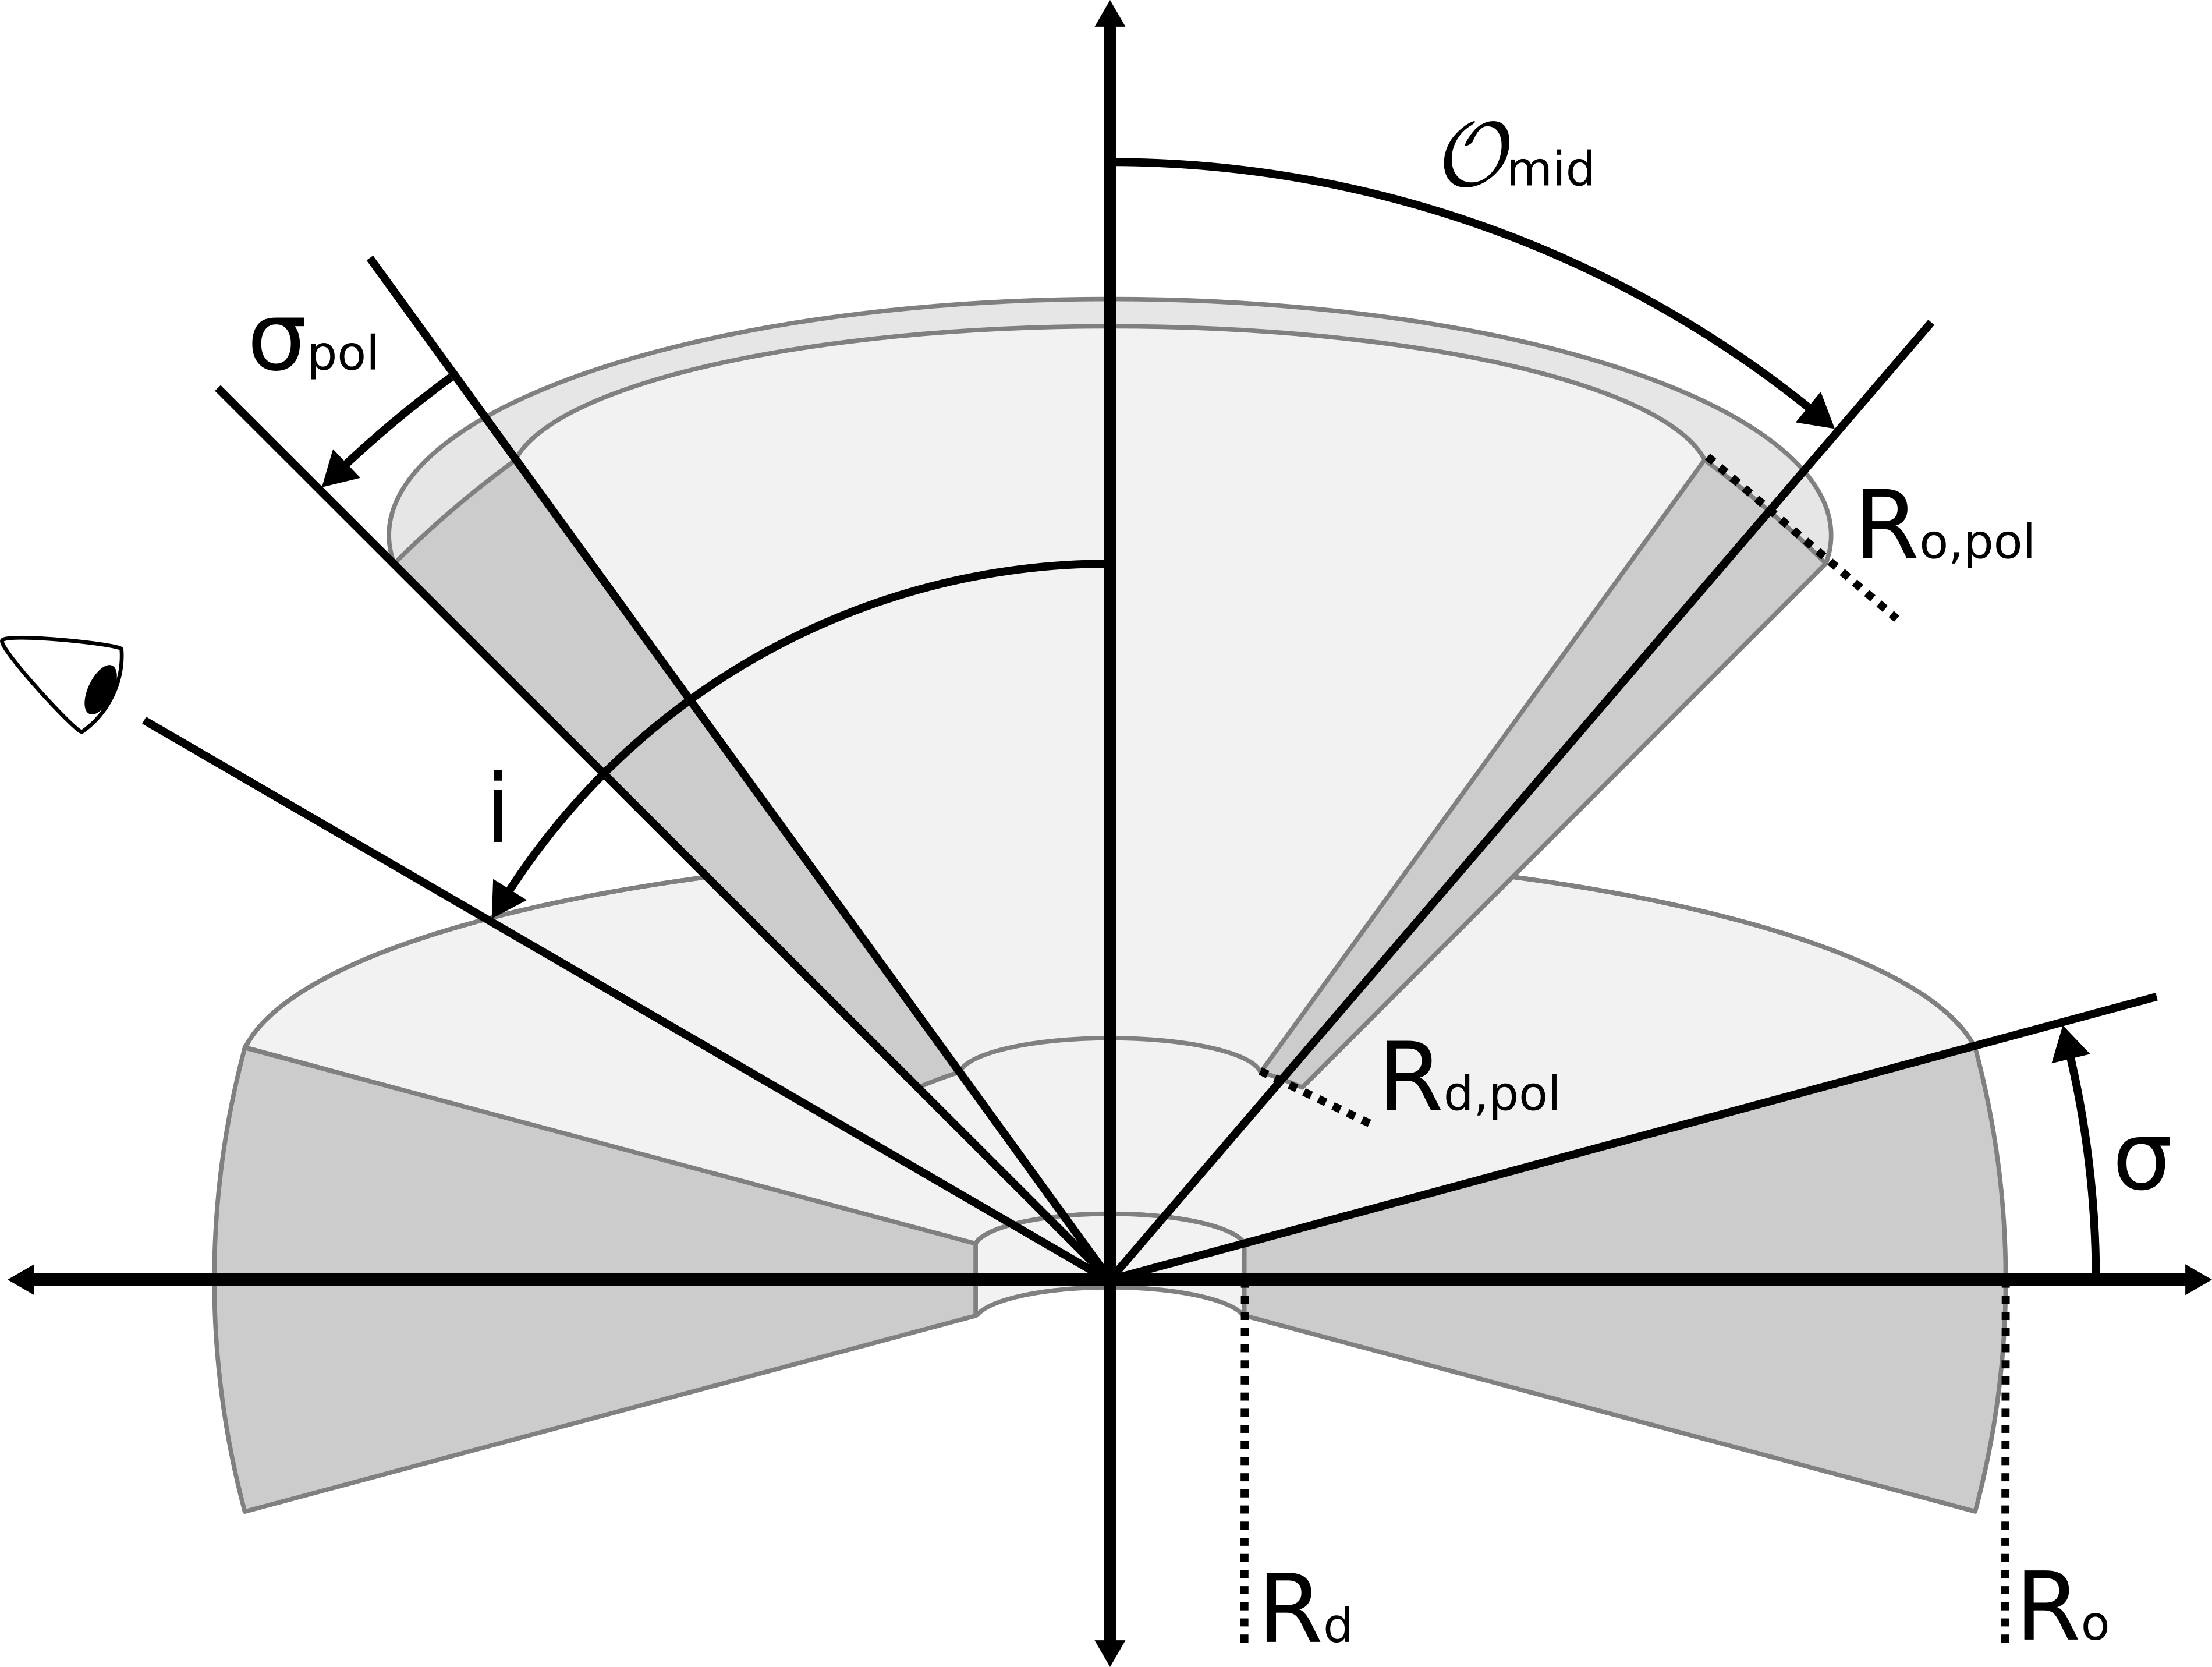
\includegraphics[width=\columnwidth]{parameter_summary.png}
 \caption{}
 \label{fig:parameter_summary}
\end{figure}

% \par Radially from the central source, clouds in both structures are arranged following a power-law distribution with index $p$ (and $p_{\text{pol}}$, for disambiguation). In polar angle ($\theta$), the clouds in the torus follow a Gaussian distribution centered in the equatorial plane. Also in polar angle ($\theta$), the bi-cone's clouds follow a Gaussian distribution centered at the opening angle $\mathcal{O}_{mid}$). The standard deviation of both Gaussian distributions are defined by $\sigma$ (or $\sigma_{pol}$) for the torus and bi-cone, respectively. The sizes of the clouds in each structure are defined by the volume filling factor $\Phi$ \& $\Phi_{pol}$, which is defined by fraction of the volume of all of the clouds in that dust structure. If $\Phi$ = 0.01, 1\% of the torus’ volume will be taken up by clouds. 
\par The dust clouds are heated either directly by the UV/optical continuum emitted from the accretion disk or, if shadowed \zach{what is shadowing?}, indirectly by the diffuse radiation field produced by the directly illuminated clouds. The illuminating AGN radiation field may be anisotropic, due to “edge darkening” of the accretion disk. Therefore, the AGN luminosity is assumed to have the following polar angle dependence:
$$L(\theta) = \left[s + (1 - s)(1/3)(1 + 2 \cos{\theta})\cos{\theta}\right]L_{\text{AGN}}$$
(see Netzer 1987), where $L_{\text{AGN}}$ is the isotropic bolometric luminosity of the AGN and the "softening parameter" $s$ determines the degree of anisotropy with an $s$ value of 1.0 corresponding to isotropic illumination. In the isotropic case, $R_d$ is a constant value, only dependent on the dust's sublimation temperature $T_{\text{sub}}$. However, in the anisotropic case $s < 1$, $R_d$ is instead a function of both the dust sublimation temperature, $T_{\text{sub}}$, and $\theta$. For the purposes of calculating $R_o$, the isotropic $R_d$ is always used in the expression of \Y.

[{\bf Insert brief overview of new grain stuff}] \zach{This needs to contain a reference to sebs paper so we can talk about the cloud grids.} \zach{Also needs to have the dust sublimation radius equation}

% From A20: The dust grain composition is a standard Galactic ISM mix of 53\% silicates and 47\% graphites assuming the Mathis-Rumpl-Nordsieck (Mathis et al. 1977) grain size distribution. Given an input AGN optical light curve, the observed cloud emission is determined by taking into account the AGN illumination (which may be anisotropic), light-travel delays within the torus, cloud shadowing, and cloud occultation effects. The torus luminosity at selected IR wavelengths is computed at each observer time step by summing over all clouds in order to produce an IR light curve for each wavelength. The TORMAC model parameters are summarized in Table 1, which also lists the values of those parameters used in the simulations presented in this paper. The models discussed in Sections 4 and 5 explore specific axes of the multi-dimensional parameter space rather than sampling all possible combinations. Therefore, we define a “standard” set of parameter values, which are the values of the parameters that are held fixed when other parameters are varied. These are indicated in bold type in the table.

\par TORMAC also calculates the anisotropic emission from individual clouds, as the illuminated face of a cloud will have a higher temperature than the non-illuminated side, see Section 2.4 of \cite{almeyda_modeling_2017}. Additionally, the emission from any given cloud is also subject to two “global” opacity effects. The first is cloud shadowing, whereby an outer cloud has its line of sight to the central AGN continuum source blocked by one or more inner clouds, closer to the central source. Clouds that are shadowed in this way are heated indirectly by the diffuse radiation emitted by surrounding directly illuminated clouds (see \cite{almeyda_modeling_2017}). Between \cite{almeyda_modeling_2020} and this paper, the implementation of cloud shadowing in TORMAC has changed, and is described in detail in Section~\ref{sec:cloudcounting}. The second is cloud occultation, whereby the emitted spectrum of a cloud may be attenuated by clouds intervening along the line of sight to the observer (see Section 2.1 in \cite{almeyda_modeling_2020}). \zach{I definitely think this paragraph should move before the description of illumination, thoughts?}

\subsubsection{Modified Cloud Shadowing}  \label{sec:cloudcounting}

\par In \cite{almeyda_modeling_2017,almeyda_modeling_2020}, an analytic approximation is used to calculate the probability that a cloud at a given radius will be shadowed. While this approximation may be sufficient for many cases, it often overestimates the number of clouds shadowed, with some extreme cases exacerbating this effect. In the past, TORMAC has used this probabilistic approach to reduce model execution time, but due to general improvements in TORMAC's model execution time, it has become computationally feasible to accurately determine which clouds are shadowed.

We compute each cloud's shadow as a cone that extends from its surface to infinity with a constant solid angle as observed from the central source. To determine if a given cloud is shadowed, we determine which of these cones the cloud intersects, and the area of intersection is calculated and summed. A cloud is considered shadowed if its intersection area is greater than 50\% of its total area. If a cloud is considered shadowed, it will only be illuminated by diffuse radiation, whereas if it is not shadowed, it will only be directly illuminated by the central source. \zach{Make clear that intersection area must be greater than 50\% for an individual cone not the sum} For shadowed clouds, the total intersection area is then used to compute the cloud's attenuated radius from the central source according to the equation
$$R_{\text{att}} = R_{\text{cl}} \cdot \exp{\left(A_{\text{int}}/2A_{\text{cl}}\right)}$$
where $R_{\text{cl}}$ is the physical radius from the central source of the cloud, $A_{\text{int}}$ is the total intersection area, and $A_{\text{cl}}$ is the area of the cloud. The attenuated radius is then used to determine the amount of diffuse radiation expected, based off of a precomputed cloud grid. \zach{What is this precomputed grid? Say that it is based off of the clouds distance and wavelength} \zach{need to better explain what the "attenuated radius" means}

\subsection{MCMC Model Fitting Using tormacFit} \label{sec:tormacFit}

\zach{Would probably be better to say something along the lines of: To rapidly sample the goodness of fit of our models across the parameter space to the ground truth observed data, we use mcmc...}As a way to estimate the constraints on the parameters for which we generate TORMAC models, we employ Markov Chain Monte Carlo (MCMC) modeling to fit the IR response models generated by TORMAC to the observations. We use a code entitled tormacFit, which is a heavily modified version of clumpyDREAM \citep{sales_embedded_2015}, to perform the MCMC search. \zach{Probably should just cite pydream} The fitter calculates the likelihood using a $\chi^2$ test using all of the points in the observed light curve. \zach{Can revise this to better show mathematically what our log liklihood looks like} Since TORMAC is capable of calculating light curves for multiple wavelengths, and multiple observed wavebands (J, H, and K) are available for NGC 3783, tormacFit was made to handle multi-wavelength fitting. The likelihoods calculated for each wavelength are multiplied to arrive at the final likelihood used for the MCMC search. \zach{Can just say that the code jointly fits the wavelengths} For all of the posterior distributions presented in Section \ref{sec:results}, we fit to both the H and K bands. We were unable to properly fit the light curves to the J band, explained in Section \ref{sec:discussion}. \zach{This is a poor location to put this info...}

We introduce two additional parameters to our MCMC search: log(amp) and Sys. Unc. (\%). The log(amp) parameter is a monochromatic scaling factor applied to the model lightcurve, used to . log(amp) values far from unity represent limitations of TORMAC to reproduce the true observed flux, or additional sources of extinction which have not been considered. The Sys. Unc. (\%) parameter is systematic uncertainty added to the uncertainty on the fluxes for the observed light curve, and represents additional random, yet unexplained fluctuations introduced during reprocessing of the optical radiation. \zach{this is not a good way to explain systematic uncertainty}

To perform the MCMC search, we calculate a set of TORMAC models which sample the parameter space on a regular grid. For MCMC proposal evaluations which do not lie on one of these grid points, the model light curve is nd-linearly interpolated between adjacent grid points. Therefore, we impose that all of our model grids are “regular”, meaning that the set of models we run is the cartesian product of all of the sets containing a respective parameter’s values to be tested, i.e., there are no gaps in the grid. 